\documentclass[journal,12pt,twocolumn]{IEEEtran}

\usepackage{setspace}
\usepackage{gensymb}
\singlespacing
\usepackage[cmex10]{amsmath}

\usepackage{amsthm}

\usepackage{mathrsfs}
\usepackage{txfonts}
\usepackage{stfloats}
\usepackage{bm}
\usepackage{cite}
\usepackage{cases}
\usepackage{subfig}

\usepackage{longtable}
\usepackage{multirow}

\usepackage{enumitem}
\usepackage{mathtools}
\usepackage{steinmetz}
\usepackage{tikz}

\usepackage{circuitikz}
\usepackage{verbatim}
\usepackage{tfrupee}
\usepackage[breaklinks=true]{hyperref}
\usepackage{graphicx}
\usepackage{tkz-euclide}

\usetikzlibrary{calc,math}
\usetikzlibrary{automata, positioning}
\usepackage{listings}
    \usepackage{color}                                            %%
    \usepackage{array}                                            %%
    \usepackage{longtable}                                        %%
    \usepackage{calc}                                             %%
    \usepackage{multirow}                                         %%
    \usepackage{hhline}                                           %%
    \usepackage{ifthen}                                           %%
    \usepackage{lscape}     
\usepackage{multicol}
\usepackage{chngcntr}

\DeclareMathOperator*{\Res}{Res}

\renewcommand\thesection{\arabic{section}}
\renewcommand\thesubsection{\thesection.\arabic{subsection}}
\renewcommand\thesubsubsection{\thesubsection.\arabic{subsubsection}}

\renewcommand\thesectiondis{\arabic{section}}
\renewcommand\thesubsectiondis{\thesectiondis.\arabic{subsection}}
\renewcommand\thesubsubsectiondis{\thesubsectiondis.\arabic{subsubsection}}


\hyphenation{op-tical net-works semi-conduc-tor}
\def\inputGnumericTable{}                                 %%

\lstset{
%language=C,
frame=single, 
breaklines=true,
columns=fullflexible
}
\begin{document}

\newcommand{\BEQA}{\begin{eqnarray}}
\newcommand{\EEQA}{\end{eqnarray}}
\newcommand{\define}{\stackrel{\triangle}{=}}
\bibliographystyle{IEEEtran}
\raggedbottom
\setlength{\parindent}{0pt}
\providecommand{\mbf}{\mathbf}
\providecommand{\pr}[1]{\ensuremath{\Pr\left(#1\right)}}
\providecommand{\qfunc}[1]{\ensuremath{Q\left(#1\right)}}
\providecommand{\sbrak}[1]{\ensuremath{{}\left[#1\right]}}
\providecommand{\lsbrak}[1]{\ensuremath{{}\left[#1\right.}}
\providecommand{\rsbrak}[1]{\ensuremath{{}\left.#1\right]}}
\providecommand{\brak}[1]{\ensuremath{\left(#1\right)}}
\providecommand{\lbrak}[1]{\ensuremath{\left(#1\right.}}
\providecommand{\rbrak}[1]{\ensuremath{\left.#1\right)}}
\providecommand{\cbrak}[1]{\ensuremath{\left\{#1\right\}}}
\providecommand{\lcbrak}[1]{\ensuremath{\left\{#1\right.}}
\providecommand{\rcbrak}[1]{\ensuremath{\left.#1\right\}}}
\theoremstyle{remark}
\newtheorem{rem}{Remark}
\newcommand{\sgn}{\mathop{\mathrm{sgn}}}
\providecommand{\abs}[1]{\vert#1\vert}
\providecommand{\res}[1]{\Res\displaylimits_{#1}} 
\providecommand{\norm}[1]{\lVert#1\rVert}
%\providecommand{\norm}[1]{\lVert#1\rVert}
\providecommand{\mtx}[1]{\mathbf{#1}}
\providecommand{\mean}[1]{E[ #1 ]}
\providecommand{\fourier}{\overset{\mathcal{F}}{ \rightleftharpoons}}
%\providecommand{\hilbert}{\overset{\mathcal{H}}{ \rightleftharpoons}}
\providecommand{\system}{\overset{\mathcal{H}}{ \longleftrightarrow}}
	%\newcommand{\solution}[2]{\textbf{Solution:}{#1}}
\newcommand{\solution}{\noindent \textbf{Solution: }}
\newcommand{\cosec}{\,\text{cosec}\,}
\providecommand{\dec}[2]{\ensuremath{\overset{#1}{\underset{#2}{\gtrless}}}}
\newcommand{\myvec}[1]{\ensuremath{\begin{pmatrix}#1\end{pmatrix}}}
\newcommand{\mydet}[1]{\ensuremath{\begin{vmatrix}#1\end{vmatrix}}}
\numberwithin{equation}{subsection}
\makeatletter
\@addtoreset{figure}{problem}
\makeatother
\let\StandardTheFigure\thefigure
\let\vec\mathbf
\renewcommand{\thefigure}{\theproblem}
\def\putbox#1#2#3{\makebox[0in][l]{\makebox[#1][l]{}\raisebox{\baselineskip}[0in][0in]{\raisebox{#2}[0in][0in]{#3}}}}
     \def\rightbox#1{\makebox[0in][r]{#1}}
     \def\centbox#1{\makebox[0in]{#1}}
     \def\topbox#1{\raisebox{-\baselineskip}[0in][0in]{#1}}
     \def\midbox#1{\raisebox{-0.5\baselineskip}[0in][0in]{#1}}
\vspace{3cm}
\title{Assignment 2}
\author{Sachin karumanchi-AI20BTECH11013}
\maketitle
\newpage
\bigskip
\renewcommand{\thefigure}{\theenumi}
\renewcommand{\thetable}{\theenumi}
Download all python codes from 
\begin{lstlisting}
https://github.com/sachinkarumanchi/probability_and_random_variables/blob/assignment2/assignment2.py
\end{lstlisting}
%
and latex-tikz codes from 
%
\begin{lstlisting}
https://github.com/sachinkarumanchi/probability_and_random_variables/blob/assignment2/Assignment2.tex
\end{lstlisting}
\section{Problem}
Two Players,A and B,alternately keep rolling a fair dice.The person gets a six first wins the game.Given the Player A starts the game,the probability that A wins the game.
\section{Solution}
Let $X\in\{1,2,3,4,5,6\}$ be the random variable representing out come of a dice.\\
Probability of getting a six on a fair dice
\begin{align}
\Pr(X=6) &=\frac{1}{6}
\end{align}
Probability of not getting a six on a fair dice
\begin{align}
\Pr(X\neq6)=\frac{5}{6}
\end{align}
The probability of some one wining in their $n^{th}$ trail is
    \begin{multline}
        \Pr{(X_n=6|X_k\neq6,k=1,2,3...,n-1)}\\
    =\frac{1}{6}\brak{\frac{5}{6}}^{n-1}
    \end{multline}
Let the probability of a wining the game is $\Pr{(A)}$\\
If A start's the game then A can win on odd numbered trail$(n)$\\
\begin{align}
n&=2m+1
\end{align}
Inorder for A to win B must lose in all of it's trails until A gets a six.\\
Therefore,
\begin{align}
   \Pr{(A)}&=\Pr{(X_1=6)}+\Pr{(X_3=6)}+\Pr{(X_5=6)}+....\\
    \Pr{(A)}&=\brak{\frac{1}{6}}+\brak{\frac{1}{6}\brak{\frac{5}{6}}^{2}}+\brak{\frac{1}{6}\brak{\frac{5}{6}}^{4}}...\\
    &=\frac{1}{6}\sum_{m=0}^{\infty}\brak{\frac{5}{6}}^{2m}
\end{align}
Here it became the sum of infinite terms in Geometric Progression $(r<1)$.\\
\begin{align}
    &=\frac{\frac{1}{6}}{1-\brak{\frac{5}{6}}^2}\\
    &=\frac{6}{11}\\
    \implies \Pr{(A)}&=\frac{6}{11}
\end{align}
Therefore, The probability that A wins the game=$\Pr{(A)=\frac{6}{11}}$
\\
\\
\centerline{ \textbf{State diagram of A and B}}


    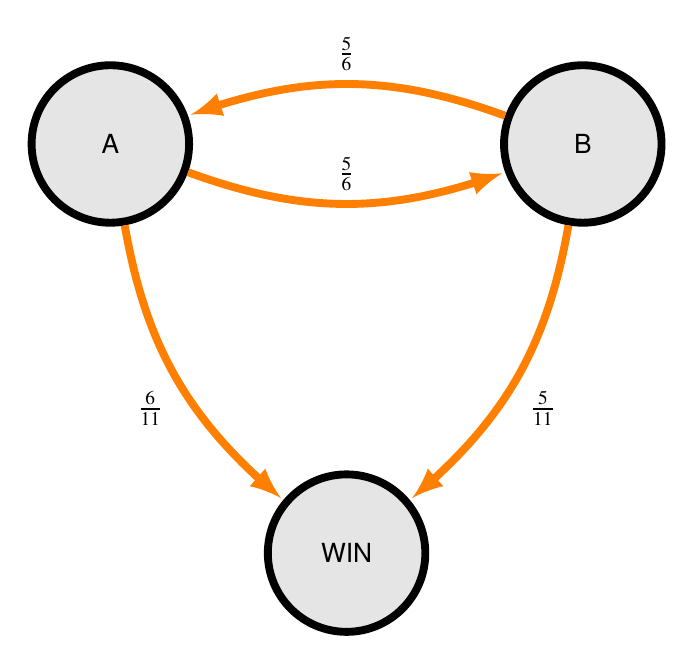
\begin{tikzpicture}[font=\sffamily]

        % Setup the style for the states
        \tikzset{node style/.style={state, 
                                    minimum width=2cm,
                                    line width=1mm,
                                    fill=gray!20!white}}

        % Draw the states
        \node[node style] at (0, 0)     (A)     {A};
        \node[node style] at (6, 0)     (B)     {B};
        \node[node style] at (3, -5.196) (WIN) {WIN};

        % Connect the states with arrows
        \draw[every loop,
              auto=right,
              line width=1mm,
              >=latex,
              draw=orange,
              fill=orange]
            (A)     edge[bend right=20]            node {$\frac{6}{11}$} (WIN)
            (A)     edge[bend right=20, auto=left] node {$\frac{5}{6}$} (B)
            (B)     edge[bend right=20]            node {$\frac{5}{6}$} (A)
            (B)     edge[bend left=20, auto=left] node {$\frac{5}{11}$} (WIN);
    \end{tikzpicture}
\end{document}